\section{The Design of UPPRESSO}
\label{sec:UPPRESSO}
This section provides the design of UPPRESSO.
We firstly present the detailed functions of identifier transformation, for trapdoor user identification and transformed RP designation.
Then, we provide an overview of UPPRESSO and describe the protocols.
Finally, we discuss the compatibility of UPPRESSO with OIDC.

\subsection{Functions of Identifier Transformation}
\label{subsec:overview}
As mentioned in Section \ref{sec:challenge},
the functions of identifier transformation
 are essential for privacy-preserving SSO systems.
In UPPRESSO,
$\mathcal{F}_{ID_{RP} \mapsto PID_{RP}}$, $\mathcal{F}_{ID_{U} \mapsto PID_{U}}$ and $\mathcal{F}_{PID_{U} \mapsto Account}$
    are constructed based on the discrete logarithm with public parameters $p$, $q$, and $g$, %% L不作为参数,我们说:e, n是RSA算法参数,不说2048是参数。
 where  $p$ is a large prime defining the finite field $GF(p)$,
 % $L$ is the length of $q$ in bits,  ($2^{L-1} < q < 2^L$)
  $q$ is a prime factor of ($p-1$), and $g$ is a generator of order $q$ in $GF(p)$.
%the prime number $q$  is the order of a multiplicative subgroup of $GF(p)$, which is generated with the generator $g$ by $\{g\ mod\ p, g^2\ mod\ p, ..., g^{q-1}\ mod\ p, 1=g^q\ mod\ p\}$.

The IdP assigns a  unique random number as  $ID_U$ ($1 < ID_U <q $) to each user,
 and a unique $ID_{RP}$ at the RP's initial registration.
$ID_{RP}$ is computed as follows, where $r$ is a random number ($1 < r < q$) generated by the IdP.

\begin{equation}
    ID_{RP} = g^{r} \bmod p
   \label{equ:IDRP}
\end{equation}


In each login,
 the user and the visited RP negotiate $PID_{RP}$ as follows.
The RP chooses a random number $N_{RP}$ ($1 < N_{RP}<q $), and the user chooses another random number $N_{U}$ ($1 < N_{U}<q $).
Then, they cooperatively compute $PID_{RP}$ as in Equation~\ref{equ:PIDRP}.

\begin{equation}
    \mathcal{F}_{ID_{RP} \mapsto PID_{RP}}: PID_{RP} = {ID_{RP}}^{N_{U} N_{RP}} \bmod p
   \label{equ:PIDRP}
   \end{equation}


$\mathcal{F}_{ID_{RP} \mapsto PID_{RP}}$ satisfies the following requirements. % described in Section~\ref{subsec:challenges}.
     %That is, the function $\mathcal{F}_{ID_{RP} \mapsto PID_{RP}}$ is invoked to generate $PID_{RP}$ for each login, while
First,
it is computationally infeasible for
    the IdP to derive $ID_{RP}$ from $PID_{RP}$ due to the discrete logarithm problem.
$N_{U}$ and $N_{RP}$  serves as nonces to ensure that (\emph{a}) $PID_{RP}$ is valid only for this login as well as the identity proof,
     and (\emph{b}) the IdP cannot correlate multiple ${PID_{RP}}$s for a same RP.
Finally,
    the cooperation by the user and the RP prevents a single malicious entity from manipulating $PID_{RP}$ in the identity proof.
%For example, the malicious user fails to make a correct RP accept a $PID_{RP}$ used in another login, while the collusive RPs fail to use a same or correlated $PID_{RP}$s for different logins.

On receiving a request of
    $ID_U$ and $PID_{RP}$ from an authenticated user,
the IdP calculates $PID_U$ as Equation~\ref{equ:PIDU},
    and binds it in the identity proof.

\begin{equation}
 \mathcal{F}_{ID_{U} \mapsto PID_{U}}: PID_U = {PID_{RP}}^{ID_U} \bmod p
 \label{equ:PIDU}
\end{equation}

% The function $\mathcal{F}_{ID_{U} \mapsto PID_{U}}$ satisfies the requirements described in Section~\ref{subsec:challenges}.
We have $PID_U = {ID_{RP}}^{N_UN_{RP}ID_U}  = g^{rN_UN_{RP}ID_U} \bmod p$ from Equations~\ref{equ:IDRP}, ~\ref{equ:PIDRP} and~\ref{equ:PIDU}.
The discrete logarithm problem ensures that the RP cannot derive $ID_U$ from $PID_U$.
Moreover,
    provided that $r$ is kept secret to the RP,
    collusive RPs cannot link a user's $PID_U$s at different RPs.
    % who can never know $r$ and $ID_U$. %have different $ID_{RP}$. %discrete logarithm of $ID_{RP}$ modulo $ID_{RP}^'$

Finally, the RP derives $Account$ for the user %with the function $\mathcal{F}_{PID_{U} \mapsto Account}$
 as Equation~\ref{equ:Account}.
Here, we define $T = (N_UN_{RP})^{-1} \bmod q$ as the trapdoor at the RP.
As $q$ is a prime number and $1< N_U, N_{RP} < q$, $q$ is coprime to $N_U N_{RP}$, and then $T$ that satisfies $T (N_U N_{RP}) = 1 \bmod q$ always exists.

\begin{equation}
   \mathcal{F}_{PID_{U} \mapsto Account}: Account = {PID_U}^{T} \bmod p
   \label{equ:Account}
   \end{equation}

We have $Account = {ID_{RP}}^{ID_U} \bmod p$ as Equation~\ref{equ:AccountNotChanged} shows,
 from Equations and \ref{equ:PIDRP}, \ref{equ:PIDU}, and \ref{equ:Account}.
So for a user's multiple logins at an RP, the RP extracts an identical $Acount$.

 \begin{multline}\label{equ:AccountNotChanged}
   Account =  {PID_{U}}^{T} = {({PID_{RP}}^{ID_U})}^{{(N_UN_{RP})^{-1} \bmod q}}\\
   = {ID_{RP}} ^ {ID_U N_U N_{RP} T \bmod q} = {ID_{RP}}^{ID_U} \bmod p
 \end{multline}

$\mathcal{F}_{PID_{U} \mapsto Account}$ satisfies the following requirements. %described in Section~\ref{subsec:challenges}.
Similar to the analysis of $PID_U$,
    the RP cannot derive $ID_U$ from $PID_U$,
        and
    collusive RPs cannot link a user's $PID_U$s at different RPs.

\noindent\textbf{Trapdoor user identification.} %is supported with these three functions.
In a user's multiple logins, the RP expresses different $PID_U$s and have corresponding $T$s,
 so that always derives the identical $Account$.
%$\mathcal{F}_{ID_{U} \mapsto PID_{U}}$ and $\mathcal{F}_{PID_{U} \mapsto Account}$
The comprehensive design of identifier transformation functions
 prevents collusive RPs from linking a user's $PID_U$s and $Account$s at different RPs, and therefore prevents RP-based identity linkage.

\noindent\textbf{Transformed RP designation.} %is also supported with $\mathcal{F}_{ID_{RP} \mapsto PID_{RP}}$ and $\mathcal{F}_{ID_{U} \mapsto PID_{U}}$, together
    % with  a user-centric verification. 放入到后面写!这里只是谈ID transformation
The $\mathcal{F}_{ID_{RP} \mapsto PID_{RP}}$ ensures that the user and RP cooperatively generate a fresh $PID_{RP}$  for a user's login,
 while $\mathcal{F}_{ID_{U} \mapsto PID_{U}}$ ensures that the IdP generates the exact $PID_U$ for the $ID_U$ who logins at $PID_{RP}$.
The IdP will bind $PID_{U}$ with $PID_{RP}$ in the identity proof, which designates this identity proof to $PID_{RP}$.
Therefore, the $PID_{RP}$ is designated to $ID_{RP}$.
Finally, the transformed RP designation is provided through the two-step designations.
The function $\mathcal{F}_{ID_{RP} \mapsto PID_{RP}}$ prevents the curious IdP from linking the $PID_{RP}$s of different logins at an RP, and therefore avoids  the  IdP-based access tracing.


\begin{table}[tb]
    \caption{The notations used in UPPRESSO.}
    \centering
%    \begin{tabular}{|c|c|c|}
    \begin{tabular}{|p{1.0cm}|p{4.5cm}|p{2cm}|}
    \hline
    {\textbf{Notation}} & {\textbf{Definition}} & {\textbf{Attribute}} \\
    \hline
    {$p$} & {A large prime.} & {Long-term constant} \\
    \hline
    {$q$} & {A large  prime factor of ($p-1$).} & {Long-term  constant} \\
    \hline
%    {$L$} & {Length of $q$. } & {Long-term} \\    \hline
    {$g$} & {A generator of order $q$ in $GF(p)$. } & {Long-term  constant} \\
     \hline
   % \hline
    %{$SK_{ID}$, $PK$} & {The private/public key to sign/verify identity proof.} & {System-unique} \\
    {$SK$, $PK$} & {The private/public key of IdP. } & {Long-term constant} \\
    \hline
    {$ID_{RP}$} & {RP's unique identifier, $ID_{RP}=g^r \bmod p$.} & {Long-term constant} \\
    \hline
%    {$r$} & {value for $ID_{RP}=g^r \bmod p$.} & {Secret, Long-term} \\
%    \hline
    {$Cert_{RP}$} & {An RP certificate. } & {Long-term constant} \\
    \hline
    {$ID_U$} & {User's unique identifier.} & {Long-term constant} \\
    \hline
    {$Account$} & {User's identifier at an RP, $Account = {ID_{RP}}^{ID_U} \bmod p$.} & {Long-term constant} \\
    \hline
    {$PID_{RP}$} & {RP's privacy-preserving identifier, $PID_{RP} = {ID_{RP}}^{N_{U} N_{RP}} \bmod p$.} & {One-time} \\
    \hline
    {$PID_U$} & {User's privacy-preserving identifier, $PID_U = {PID_{RP}}^{ID_U} \bmod p$.} & {One-time}\\
    \hline
    {$N_U$} & {User-generated random nonce for $PID_{RP}$.} & {One-time} \\
    \hline
    {$N_{RP}$} & {RP-generated random nonce for $PID_{RP}$.} & {One-time} \\
    \hline
    {$Y_{RP}$} & {Public value for $N_{RP}$, $Y_{RP} = {ID_{RP}}^{N_{RP}} \bmod p$.} & {One-time} \\
    \hline
    {$T$} & {A trapdoor, $T=(N_U N_{RP})^{-1} \bmod q$.} & {One-time} \\
    \hline
    \end{tabular}
    \label{tbl:notations}
\end{table}

\subsection{UPPRESSO Overview}
\label{implementations}
In addition to the functions of identifier transformation,
    UPPRESSO needs to introduce more steps at the user to facilitate these identifier transformations.
It is worthy noting that,
    in order to protect user privacy against both the IdP and the visited RP,
        these steps have to be conducted at the user.
Firstly,
    because the IdP is unaware of the visited RP and also the RP's endpoint to receive the identity proof,
        this endpoint shall be queried by the user from the trusted IdP indirectly.
In UPPRESSO this is implemented as an RP certificate signed by the IdP,
    which is composed of $ID_{RP}$, the RP's endpoint and other supplementary information.
The user handles the endpoint by itself.
Secondly,
    after the negotiation of $PID_{RP}$,
        it is registered at the IdP by the authenticated user.
This cannot be finished by the RP; otherwise,
    the IdP will correlate $PID_{RP}$ and $ID_{RP}$.

%user-centric verification,  both the user and RP checks the uniqueness of $PID_{RP}$, while the user further checks that $PID_{RP}$ is exactly generated for the RP $ID_{RP}$,  and then sends the identity proof  only  to this RP.

UPPRESSO runs with four procedures, including system initialization, RP initial registration, user registration and SSO login.
The system initialization is conducted only once by the IdP to establish the system.
The RP initial registration is launched by each RP to obtain the necessary configurations (a unique identifier $ID_{RP}$ and its RP certificate $Cert_{RP}$) from the IdP before it provides services for users,
    and each RP launches this procedure only once.
The user registration is launched only once by each user to set up a unique user identifier $ID_U$ and the corresponding credential.
   % where $ID_U$ is generated by the IdP and only provided to the corresponding user.
Finally, the SSO login is launched when a user attempts to log in an RP,
    and it is designed based on the functions of identifier transformation.

The procedure for user registration is the same as that in typical SSO systems.
Therefore, we focus on the procedures of system initialization, RP initial registration and SSO login.
For clarity, we list the notations in Table~\ref{tbl:notations}.

\vspace{1mm}\noindent \textbf{System initialization.} The IdP %chooses $L$,
 generates a large prime $p$, a prime factor $q$ of $p-1$
  and a generator $g$ of order $q$ as the parameters for the discrete logarithm problem. %~\cite{gallagher2013digital}.
The IdP generates one key pair ($SK$, $PK$) to sign identity proofs and RP certificates.
The lengths of $p$, $q$ and ($SK$, $PK$) shall satisfy the requirements of security strength.

The IdP keeps $SK$ secret, while $p$, $q$, $g$ and $PK$ are public parameters.
%The values of $p$, $q$, $g$ remain the same during the full lifecycle of an SSO system.
%While, the asymmetric key pair ($SK$, $PK$) will be updated when necessary. For example, when $SK$ is leaked, IdP must update ($SK$,$PK$).

\vspace{1mm}\noindent\textbf{RP initial registration.}
An RP registers itself at the IdP to request $ID_{RP}$ and $Cert_{RP}$ as follows:
\begin{enumerate}
\item RP sends a registration request to the IdP,
    including the RP's endpoint (e.g., URL) for receiving the identity proof.
\item IdP chooses a unique random number $r$ ($1 < r < q$), computes $ID_{RP} = g^r \bmod p$,
signs $[ID_{RP}, endpoint, *]$ using $SK$, where $*$ is  supplementary information such as the RP's common name,
and returns $Cert_{RP} = [ID_{RP}, endpoint]_{SK}$ to the RP, where $[\cdot]_{SK}$ means a message signed using $SK$.
\item The RP  verifies $Cert_{RP}$ using $PK$,  and then accepts $ID_{RP}$ and $Cert_{RP}$.
\end{enumerate}

Note that, $ID_{RP}$ cannot be chosen by the RP,
 and it must be chosen by the IdP and $r$ is kept unknown to the RP.
On the contrary,
    $ID_U$ may be chosen by the user or the IdP,
    provided that it is unique for each user.

\vspace{1mm}\noindent\textbf{SSO login.}
Once a user attempts to log in at an RP, the SSO login is initiated.
%We use the OIDC implicit protocol flow as an example, to demonstrate  how to integrate the three functions $\mathcal{F}_{ID_{U} \mapsto PID_{U}}$, $\mathcal{F}_{ID_{RP} \mapsto PID_{RP}}$ and $\mathcal{F}_{PID_{U} \mapsto Account}$ into the typical SSO systems.
As shown in Figure~\ref{fig:UPPRESSO}, the SSO login consists of four phases,
 RP identifier transformation,
  RP identifier refreshing,
  $PID_U$ generation and $Account$ calculation.
In the RP identifier transforming, the user and RP negotiate $PID_{RP} = {ID_{RP}}^{N_{U} N_{RP}} \bmod p$.
In the RP identifier refreshing, the user registerers $PID_{RP}$ at the IdP.
In the $PID_U$ generation, the IdP calculates $PID_U = {PID_{RP}}^{ID_U} \bmod p$ and signs the identity proof.
And in the $Account$ calculation, the RP derives $Account = {{PID_{U}}}^{{(N_UN_{RP})^{-1} \bmod q}}$ after verifying the identity proof,
    and allows the user to log in as $Account$.

\subsection{UPPRESSO Protocol flow}
\label{sebsec:loginprocess}
Figure~\ref{fig:process} shows the SSO login protocol of UPPRESSO. %the SSO login sub-protocol provides the secure SSO service and prevents both the IdP-based access tracing and RP-based identity linkage.
 % prevents the curious IdP from obtaining the RP's identifying information during the interchanges,
%  and avoids the adversary to break the security and user's privacy.
Here we introduce the detailed processes for each step in Figure~\ref{fig:process}.

\begin{figure*}
  \centering
  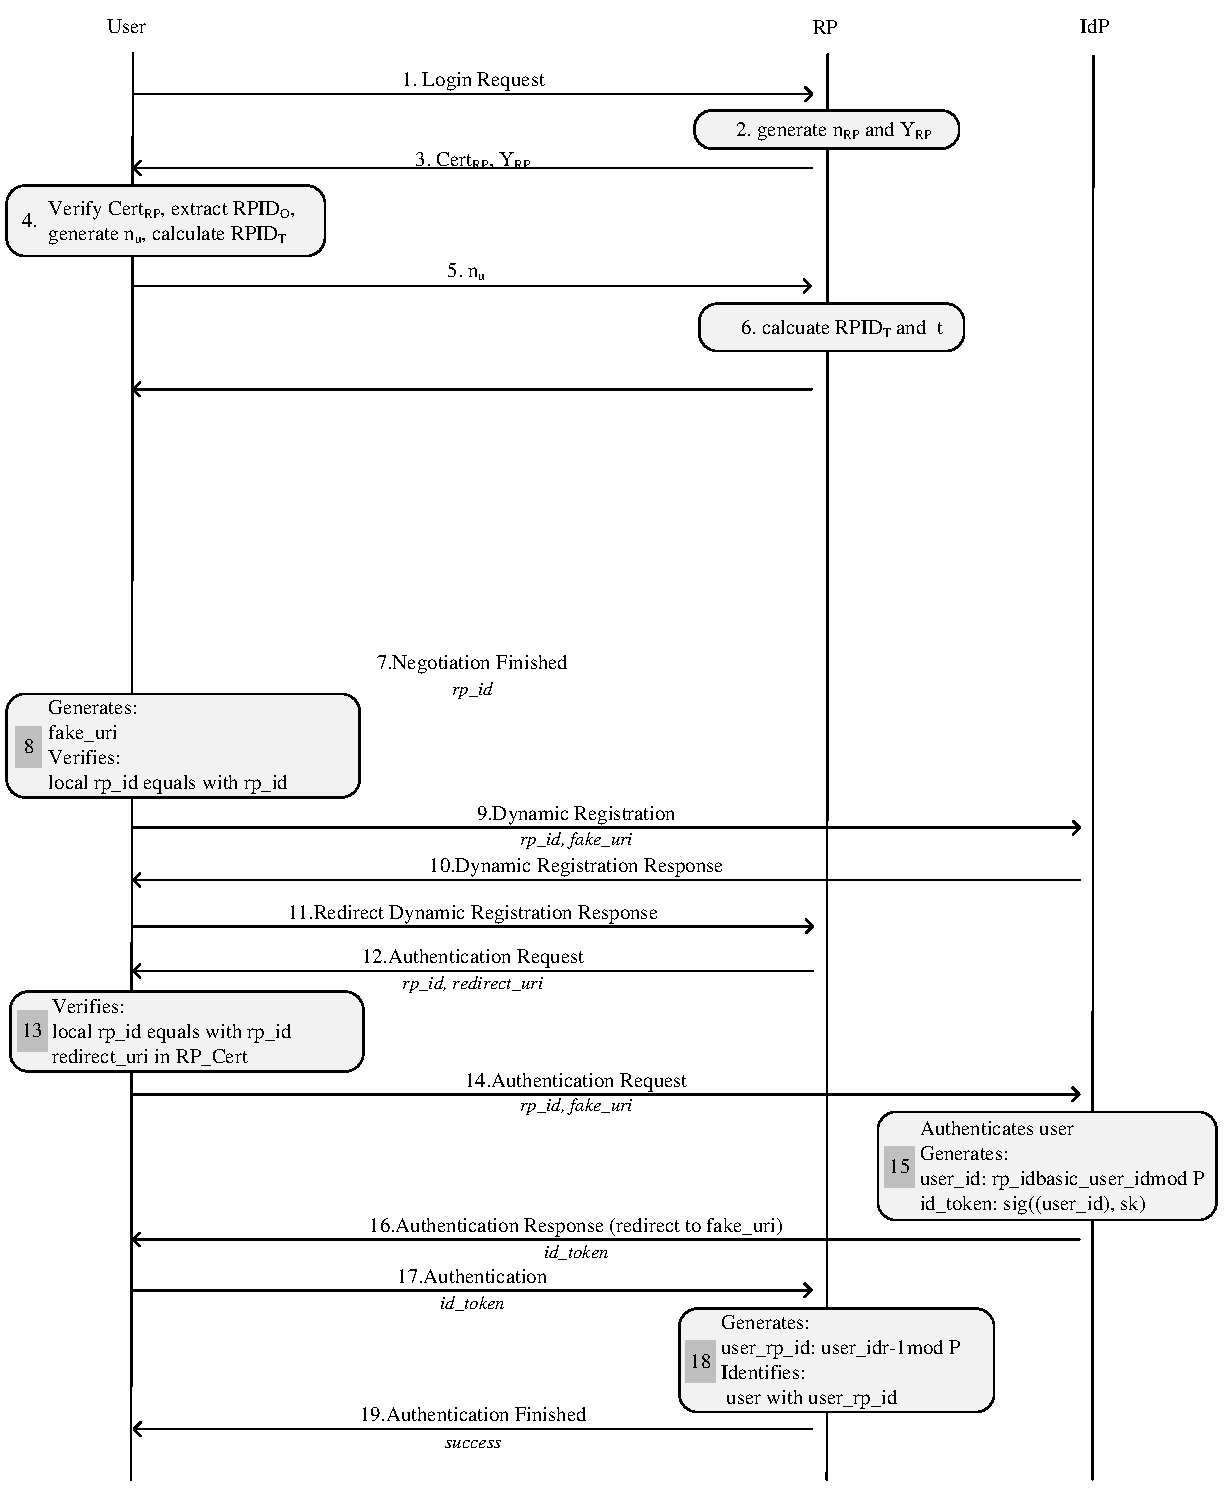
\includegraphics[width=0.85\linewidth]{fig/process.pdf}
  \caption{Process for each user login.}
  \label{fig:process}
\end{figure*}

\vspace{1mm}\noindent\textbf{RP identifier transforming.}
In this phase, the user and RP cooperative to generate $PID_{RP}$ as follows:
\begin{itemize}
  \item The user sends a login request to trigger the negotiation of $PID_{RP}$ (Step 1).
  \item The RP chooses a random $N_{RP}$ ($1 < N_{RP} <q$), calculates $Y_{RP}={ID_{RP}}^{N_{RP}} \bmod p$ (Step 2.1.1);
   and sends $Y_{RP}$ with $Cert_{RP}$  to the user (Step 2.1.2).
  \item The user checks the $Cert_{RP}$, extracts $ID_{RP}$ from the valid $Cert_{RP}$, chooses a random $N_U$ ($1 < N_U <q$) to calculate $PID_{RP}={Y_{RP}}^{N_{U}} \bmod p$ (Step 2.1.3); and sends $N_U$ %with $PID_{RP}$
       to the RP (Step 2.1.4).
  \item The RP calculates $PID_{RP}$ with $N_U$ and $Y_{RP}$, %checks its consistency with the received one,
   derives the trapdoor $T={(N_U N_{RP})}^{-1} \bmod q$ (Step 2.1.5); and 
   acknowledges the negotiation.
   %sends the calculated $PID_{RP}$ to the user (Step 2.1.6).
%  \item The user checks the consistency of the received $PID_{RP}$ with the stored one.
\end{itemize}
During the process, the user will halt the login, if  the $Cert_{RP}$ is invalid.
 %or the received $PID_{RP}$ is different from the stored one. The RP also halts the process if the $PID_{RP}$ sent by the user is inconsistent with the calculated one.
The user verifies that $PID_{RP} \neq g \bmod p$;
    if $PID_{RP} = g \bmod p$, it means that $N_U = 0 \bmod q$ or $N_{RP} = 0 \bmod q$
        and then $PID_U = {g}^{ID_U}$ is constant.

\vspace{1mm}\noindent\textbf{RP identifier refreshing.}
The user registers $PID_{RP}$ at the IdP as follows.
\begin{itemize}
  \item The user generates an one-time endpoint to hide the RP's endpoint from IdP (Step 2.2.1), and sends the RP identifier refreshing request [$Reg$, $PID_{RP}$, Hash($Y_{RP}$, $N_U$), one-time endpoint] to the IdP (Step 2.2.2).
  \item The IdP authenticates the user if necessary (Step 3); The IdP checks $PID_{RP}$, and constructs the response [$RegRes$, $RegMes$, $Sig_{Reg}$] (Step 2.2.3). The $RegRes$ is the result, and is set as $OK$ only when $PID_{RP}$ is not used with other valid and is of order $q$ module $p$. The $RegMes$ is the same as the dynamic registration response, and contains $PID_{RP}$, the issuing time and valid time. The $Sig_{Reg}$ is the signature for $RegRes$, $RegMes$ and Hash($Y_{RP}$, $N_U$) generated by the IdP with $SK$.
  \item The user accepts $RegRes$ if $PID_{RP}$ is correct and the valid signature by the IdP,
    and forwards the registration result to the RP (Step 2.2.4).
  \item The RP checks $Sig_{SK}$ and $RegMes$, and accepts $RegRes$ only when $Sig_{Reg}$ is valid, Hash($Y_{RP}$, $N_U$) and $PID_{RP}$ are the same as the negotiated one, and $RegMes$ is not expired.
\end{itemize}
If $RegRes$ is $OK$, the RP identifier refreshing completes. Otherwise, the user and RP will renegotiate the $PID_{RP}$.
Here, Hash($Y_{RP}$, $N_U$) is attached as 

The IdP check $PID_{RP}$ is unique in unexpired ones,
 otherwise, this is might be accepted by other RP (see Section xxx for details).

The RP checks if Hash($Y_{RP}$, $N_U$) matches,
    to ensure this is signed for it (not for other RPs).
More details are in xxxxx

\vspace{1mm}\noindent\textbf{$\mathbf{PID_U}$ generation.}
In this phase, the RP continues the process of the user's login and obtains the $PID_U$ generated by the IdP. The processes are as follows.
\begin{itemize}
  \item The RP uses $PID_{RP}$ and the endpoint to construct an identity proof request.  %, which is the same as the one in  OIDC.
   (Step 2.3).
  \item The user checks the consistency of the received $PID_{RP}$  with the negotiated one (Step 2.4); replaces the endpoint with the one-time endpoint generated in Step 2.2.1, and sends the modified identity proof request to the IdP (Step 2.5).
  \item The IdP authenticates the user if necessary (Step 3); 
  The IdP checks whether $PID_{RP}$ and the one-time endpoint have been registered and unexpired,
   calculates $PID_U = {PID_{RP}}^ID_U \bmod p$,  constructs the identity proof [$PID_{RP}$, $PID_U$, $ValTime$, $Attr$,$Sig_{IdProof}$] where $ValTime$ is the valid period, $Attr$ contains the  attributes that the user agrees to provide to the RP,
    $Sig_{IdProof}$ is the signature of the identity proof generated by IdP with $SK$ (Step 4). Then, the IdP sends the identity proof with the one-time endpoint to the user (Step 5.1).
  \item The user finds  the  endpoint corresponding to the one-time endpoint (Step 5.2),
   and forwards the identity proof to the RP through this endpoint (Step 5.3).
\end{itemize}
The user halts the process if the $PID_{RP}$ in the identity proof request is inconsistent with  the negotiated one.
The IdP rejects the identity proof request, if the $PID_{RP}$ and the one-time endpoint have not been registered.


\vspace{1mm}\noindent\textbf{$\mathbf{Account}$ calculation.}
Finally, RP derives the user's  $Account$ and completes the user's login as follows. The RP performs the checks on the identity proof, including the valid time, correctness of $Sig_{IdProof}$, and   the consistency between $PID_{RP}$ and the  negotiated one. If all the checks pass, the RP extracts $PID_U$, and calculates $Accout = {PID_U}^T \bmod p$ (Step 6); and sends the $Success$ as the login result to the user (Step 7). If any check fails, the RP returns the $Fail$ to the user.

\begin{figure}[t]
  \centering
  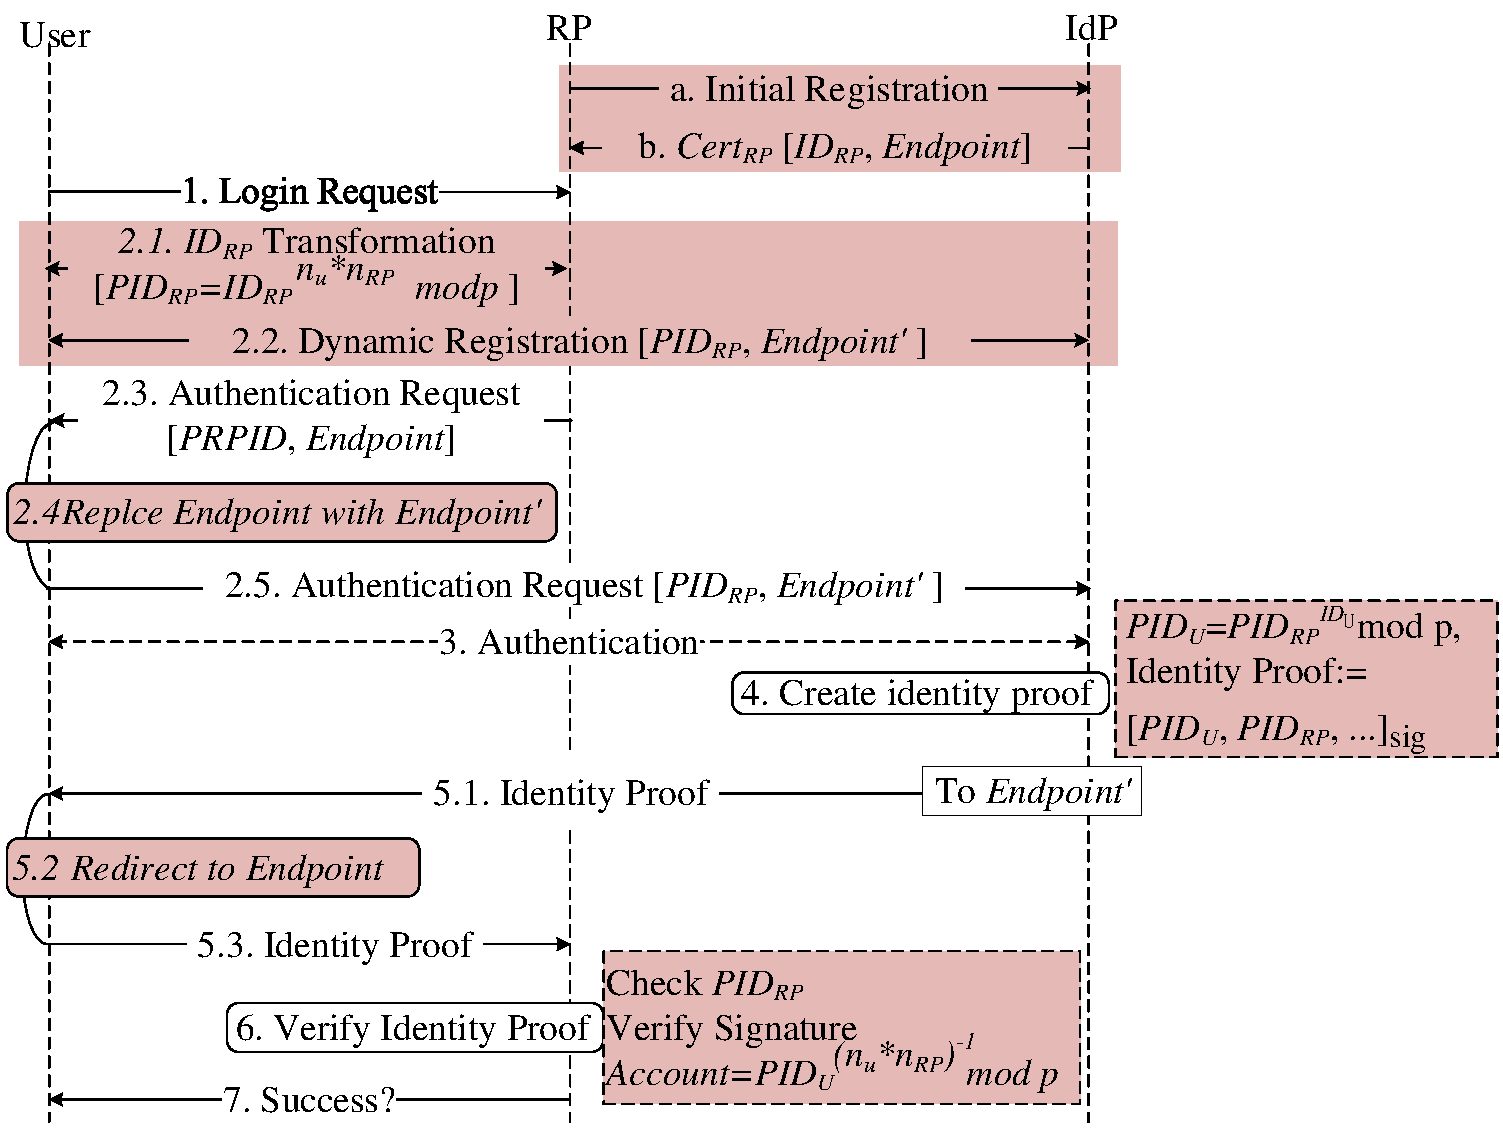
\includegraphics[width=\linewidth]{fig/overview1.pdf}
  \caption{UPPRESSO compatibility with OIDC.}
  \label{fig:UPPRESSO}
\end{figure}

\subsection{Compatibility with OIDC}
\label{subsec:compatible}
UPPRESSO could be integrated in the traditional SSO systems, to  prevent the IdP-based access tracing and RP-based identity linkage.
The integration doesn't degrade the security and only requires minimal modification.
Here, we use the implicit protocol flow of OIDC as an example to demonstrate the compatibility of UPPRESSO with the traditional SSO systems, as shown in Figure~\ref{fig:UPPRESSO}.
The further analysis, such as integration with the authorization code flow of OIDC,  is provided in Section~\ref{sec:discussion}.

UPPRESSO doesn't introduce any new role, nor change the security assumptions on each role (i.e., user, IdP and RP).

As shown in Figure~\ref{fig:UPPRESSO}, in UPPRESSO, the SSO protocol for identity proof  (Steps between 2.3 and 7) is the same as in OIDC (Steps between 2 and 7); the formats of identity proof and corresponding request are the same as in OIDC; the correctness checks on the identity proof request at the IdP (i.e., consistency of RP' identifier and endpoint with the registered one) are the same as in OIDC; the correctness checks on the identity proof (i.e., consistency of RP' identifier with the one in the request, integrity, validity time, freshness, and etc.) at the RP are the same as in OIDC.

%以下为描述Step 2.3到7的详细内容.
%That is, the RP construct a request for identity proof (Step 2.3); the user redirects this request to the IdP (Step 2.5); the IdP generates the identity proof (Step 4), and sends it to the user (Step 5.1) who redirects it to the RP (Step 5.3); and finally the RP verifies the identity proof (Step 6).

However, UPPRESSO achieves privacy preservation by integrating  $\mathcal{F}_{ID_{U} \mapsto PID_{U}}$, $\mathcal{F}_{ID_{RP} \mapsto PID_{RP}}$ and $\mathcal{F}_{PID_{U} \mapsto Account}$, and  introduces the following modifications on OIDC.

\begin{enumerate}
  \item The identity proof is bound with $PID_{RP}$ instead of $ID_{RP}$, which introduces the RP identifier transforming (Step 2.1)  and RP identifier refreshing (Step 2.2).
  \item The identity proof is designated to one-time endpoint instead of RP's identifying endpoint, which requires the user to register the one-time endpoint in Step 2.2 and replace it with the original endpoint in Step 5.2.
  \item IdP generates $PID_U$ based on ($PID_{RP}$, $ID_U$) instead of ($ID_{RP}$, $ID_U$).
  \item The RP calculates $Account$ from the changing $PID_U$ instead of an unchanged one.
\end{enumerate}

%上述modification如何实现的,简单描述
%to add: PID_{RP} transforming 和 RP identifer refreshing在user和RP的页面自己完成了。 都用现成的数据格式
%one-time endpoint 和endpoint
The above modifications could be completed automatically for each login, without affecting other communication pattern.
The user automatically invokes the JavaScript functions to complete RP identifier transforming, one-time endpoint generating/replacing and RP identifier refreshing for each login. While, the RP server and IdP server provide the corresponding web service to complete the processing automatically.
The protocol of RP identifier transformation is based Diffie-Hellman key exchange~\cite{DiffieH76}, while $N_U$ is provided to RP for computing the trapdoor.
The protocol of RP identifier refreshing is based on the dynamic registration in OIDC, while it is triggered by the user instead of the RP, adds $PID_{RP}$ in the request and includes a signature $Sig_{Res}$ in the response.

\begin{comment}
\vspace{1mm}\noindent \textbf{Consistency with OIDC.}
As shown in Figure~\ref{fig:UPPRESSO}, the architecture of UPPRESSO is the same as the one in OIDC. UPPRESSO does not introduce any new entity, but only integrates the three function $\mathcal{F}_{ID_{U} \mapsto PID_{U}}$, $\mathcal{F}_{ID_{RP} \mapsto PID_{RP}}$ and $\mathcal{F}_{PID_{U} \mapsto Account}$ into the processes at the IdP, RP, and user.

The formats of the  identity proof and corresponding request, and the verification of the identity proof,  are almost same in OIDC and UPPRESSO.
The only difference is that $ID_{RP}$ and endpoint are replaced with the privacy-preserving versions, i.e., $PID_{RP}$ and one-time endpoint, in UPPRESSO.
As $PID_{RP}$ is also unique and corresponds exactly to $ID_{RP}$, and one-time endpoint corresponds to the RP's endpoint correctly,
 the binding, integrity and confidentiality of identity proof will also be ensured in UPPRESSO, and there is no degradation on the security of OIDC.

\vspace{1mm}\noindent \textbf{Minimal modification to OIDC.}
UPPRESSO only requires small modification on OIDC to integrate $\mathcal{F}_{ID_{U} \mapsto PID_{U}}$, $\mathcal{F}_{ID_{RP} \mapsto PID_{RP}}$ and $\mathcal{F}_{PID_{U} \mapsto Account}$.
For $\mathcal{F}_{ID_{U} \mapsto PID_{U}}$ and $\mathcal{F}_{PID_{U} \mapsto Account}$, we directly use them to replace original functions for $PPID$ at the IdP and the $Account$ at the RP.
For $\mathcal{F}_{ID_{RP} \mapsto PID_{RP}}$, we inject a negotiation process and a dynamic registration for each SSO login,
 where the negotiation process between the user and RP generates a $PID_{RP}$,
  while the dynamic registration is used to check the uniqueness of $PID_{RP}$.
In UPPRESSO, the dynamic registration is slightly modified as follows: an RP identifer ($PID_{RP}$)  is added in the request, and a signature ($Sig_{Res}$)  is included in the response for its verification at the RP.
\end{comment}




